\documentclass[xcolor=svgnames,handout]{beamer}

\usepackage[utf8]    {inputenc}
\usepackage[T1]      {fontenc}
\usepackage[english] {babel}

\usepackage{hyperref}
\usepackage{csquotes}
\usepackage{amsmath,amsfonts,graphicx}
\usepackage{beamerleanprogress}
\usepackage[
backend=biber,
style=alphabetic,
sorting=ynt
]{biblatex}
\addbibresource{credits.bib}

\title[JD\hspace{2em}] {Jack Dorsey}

\author{Adrian Lucr\`{e}ce C\'{e}leste}

\date{\today}

\institute{Norwich High School}

\setbeamertemplate{navigation symbols}{\insertframenavigationsymbol{}\insertsectionnavigationsymbol{}\insertbackfindforwardnavigationsymbol{}}
\begin{document}
\section{Introduction}

\subsection{Intro slide}
\maketitle


\subsection{Table of Contents}

\begin{frame}[allowframebreaks]{Table of Contents}
	\tableofcontents
\end{frame}

\subsection{Background info}
\begin{frame}{Background info}
\begin{itemize}
    \item Jack Dorsey was born in St.\ Louis, Missouri.~\cite{timleonard2009}~\cite{lisabrown2010}
    \begin{itemize}
        \item{Parents:} Tim Dorsey, and Marcia Smith~\cite{markglaser2007}~\cite{porandrewchernin2009}~\cite{timbarker2009}
        \end{itemize}
        \item{Highschool:} Bishop DuBourg High School~\cite{markglaser2007}
%        \item Dorsey became interested in Dispatch Routing at age 14~\cite{markglaser2007}
        \item{Colleges Attended:}
        \begin{itemize}
            \item Missouri University of Science and Technology~\cite{unkown2009}
            \item Dorsey later transferred to the New York University Tandon School of Engineering~\cite{unkown2009}
            \item Dorsey ended up dropping out of NYUTSoE~\cite{unkown2009}
        \end{itemize}
    \end{itemize}
	\begin{figure}[h]
		\centering
		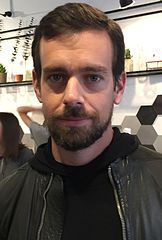
\includegraphics[scale=0.25]{Dorsey.jpg}
		\caption{Dorsey, 2014~\cite{cellanr2014}}
	\end{figure}
\end{frame}

\section{Twitter}

\subsection{Inspiration}

\begin{frame}
{Inspiration}
  \begin{itemize}
      \item{Dorsey's interest in dispatch routing grew at age 14~\cite{markglaser2007}}
      \item{Dorsey Initially had thoughts about twitter while at NYU~\cite{unkown2009}}
      \item{While Dorsey worked on dispatching as a developer, he moved to California~\cite{businessweek2008}~\cite{jackdorsey2009}}
      \item While at Oakland, CA, Dorsey started a dispatching company that functioned on the web~\cite{jackdorsey2006}.
  \end{itemize}
	\begin{figure}[h]
		\centering
		
\includegraphics[scale=0.15]{lightbulb.png}
		\caption{\cite{anonymous2014}}
	\end{figure}
\end{frame}

\subsection{Prototype}
\begin{frame}{Prototype}
	\begin{itemize}
		\item Inspired by
			\begin{itemize}
				\item AOL Instant Messenger~\cite{jackdorsey2006}
				\item Livejournal~\cite{jackdorsey2006}
			\end{itemize}
		\item Dorsey approached Odeo.
			\begin{itemize}
				\item With the help of Biz Stone, a prototype of twitter was built in two weeks~\cite{markglaser2007}
			\end{itemize}
			\item Many users were attracted from Odeo~\cite{markglaser2007}
			\item Evan Williams ended up investing~\cite{markglaser2007}
	\end{itemize}
	\begin{figure}[h]
		\centering
		
\includegraphics[scale=0.10]{twitter-logo.png}
		\caption{\cite{enow2011}}
	\end{figure}
\end{frame}

\subsection{Obvious Corporation}

\begin{frame}
{Obvious Corporation}
	\begin{itemize}
		\item Obvious Corporation was co-founded by:~\cite{markglaser2007}~\cite{patrickhoge2011}
			\begin{itemize}
				\item Biz Stone
				\item Evan Williams
				\item Jack Dorsey
				\item Noah Glass
			\end{itemize}
		\item Obvious Corporation spun off Twitter Inc.~\cite{markglaser2007}~\cite{patrickhoge2011}
			\begin{itemize}
				\item With Jack Dorsey as CEO
				\item Dorsey went through two rounds of funding
					\begin{itemize}
						\item Funding was provided by Venture capitalists~\cite{clairecainmillervindugoel2008}
					\end{itemize}
				\item Dorsey lost his job as CEO~\cite{kevinroose2013}
					\begin{itemize}
							\item He would leave work early to pursue fashion and yoga
					\end{itemize}
			\end{itemize}
	\end{itemize}
	\begin{figure}[h]
		\centering
		
\includegraphics[scale=0.10]{bills_and_coins-edit.png}
		\caption{\cite{historicairUnknown}}
	\end{figure}
\end{frame}

\section{Analysis}

\subsection{Impact}

\subsubsection{Economically}
\begin{frame}{Impact: Economically}
	\begin{itemize}
		\item Personally I don't think twitter was intended to make money
		\item Twitter eventually did end up starting a number of advertising systems
			\begin{itemize}
				\item Twitter has paid advertising for companies in the form of ``promoted tweets''~\cite{charlesarthur2010}~\cite{sarakimberley2010}
				\item Twitter has an agreement with the World Entertainment News Network~\cite{olivierlaurent2011}
				\item Twitter also has a self advertising service for small businesses~\cite{todowasserman2011}~\cite{zachminers2013}~\cite{todowasserman2012}
				\item A feature called ``Instant Unlock' was introduced, which rewards people for tweeting about brands.~\cite{martyswant2016}
			\end{itemize}
	\end{itemize}
	\begin{figure}[h]
		\centering
		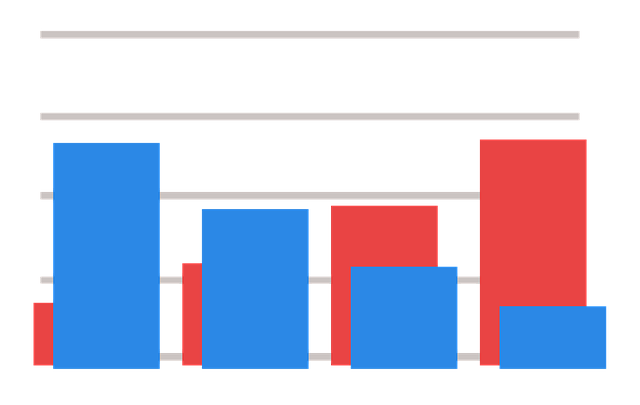
\includegraphics[scale=0.15]{clipartgraph.png}
		\caption{\cite{artsybeeUnknown}}
	\end{figure}
\end{frame}

\subsubsection{Socially}
\begin{frame}
{Impact: Socially}
	\begin{itemize}
		\item Socially Twitter has had quite the impact on the world,
			\begin{itemize}
			\item The service has been used as a form of civil disobedience~\cite{haroonsiddique2010}~\cite{adamgabbattmatthewtaylor2011}
			\item It has been used as a ``weapon''~\cite{ricardobuettnerkatharinabuettner2016}
			\item Also Twitter has been used as an emergency communication service.~\cite{alexandermillsruichenjinkyuleehraghavrao2009}~\cite{chelseajcartergregbotelho2013}~\cite{brookejarvis2013}~\cite{robertpowerbellarobinsondavidratcliffe2013}~\cite{paulsearledanielcbowdenmichelleguy2013}
			\end{itemize}
	\end{itemize}
	\begin{figure}[h]
		\centering
		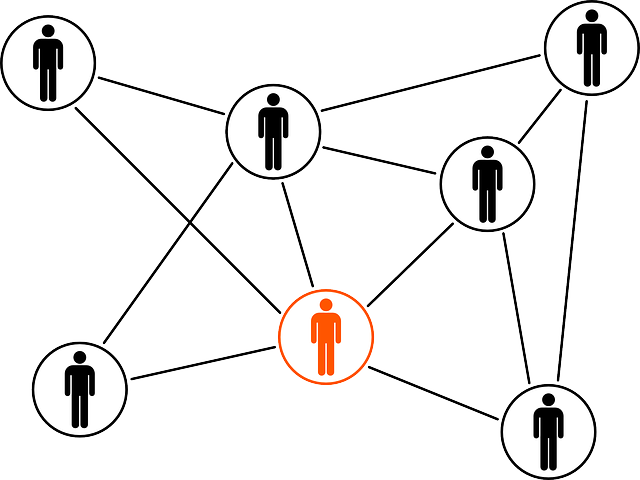
\includegraphics[scale=0.15]{social-vector.png}
		\caption{\cite{openclipartvectorsUnkown}}
	\end{figure}

\end{frame}

\subsubsection{Perhaps not so positively}
\begin{frame}
{Impact: Perhaps not so positively}
	
	\begin{itemize}
		\item Some Critics felt like it was just a fad, like ``CB Radio'' had been.~\cite{johncdvorak2009}
		\item Other Critics said they felt ``too'' connected on twitter.~\cite{andrewlavallee2007}
		\item Twitter has also allegedly banned a pro Bernie Sanders account~\cite{getthewordout2016}
	\end{itemize}
	\begin{figure}[h]
		\centering
		
\includegraphics[scale=0.15]{thumb-down.png}
		\caption{\cite{openclipartvectors}}
	\end{figure}

\end{frame}

\subsubsection{Today}

\begin{frame}{Impact: Today!}
	\begin{itemize}
	\item Disclaimer: opinions ahead
		\begin{itemize}
			\item Twitter is still used, maybe not as heavily as it once was when it first started.
			\item Twitter can have a huge impact on the economy by:
				\begin{itemize}
					\item Quickly, and responsively: posting new shocking events
					\item Adding to the promotion of small business
					\item Adding to the promotion of big business
				\end{itemize}
			\item Rather then evolving into segregated products twitter has:
				\begin{itemize}
					\item Used and created Open-Source programs~\cite{twitter}~\cite{twitter2013}~\cite{twittergithub2013}~\cite{twitterwebarchive22013}
					\item Created an Effective ecosystem so that twitter can evolve
				\end{itemize}
		\end{itemize}
	\end{itemize}
	\begin{figure}[h]
		\centering
		
\includegraphics[scale=0.10]{clock.png}
		\caption{~\cite{clkerfreevectorimagesUnknown}}
	\end{figure}
\end{frame}

\subsection{Net Worth}

\begin{frame}{Net Worth}
	\begin{itemize}
		\item Twitter is now a Public Traded Company
			\begin{itemize}
				\item Twitters first announced this September 12, 2013~\cite{leokelion2013}
				\item When released, shares were priced at \$26 USD~\cite{aaronpressman2013}
				\item The stock ticker is NYSE:~TWTR~\cite{nyse2016}
			\end{itemize}
	\end{itemize}
	\begin{figure}[h]
		\centering
		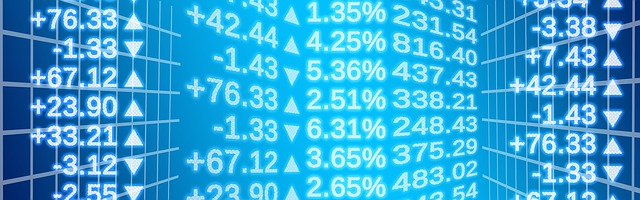
\includegraphics[scale=0.25]{stock-market.jpg}
		\caption{\cite{geraltUnknown}}
	\end{figure}
\end{frame}

\subsection{Spending}

\begin{frame}{Spending}
	\begin{itemize}
		\item Dorsey is on the record for donating to the Democratic party~\cite{opensecrets.org2010}
		\item Dorsey also developed Square, Inc.~\cite{square2010}~\cite{jessihempel2011}
		\item Twitter is a publicly traded company~\cite{leokelion2013}~\cite{aaronpressman2013}~\cite{nyse2016}
	\end{itemize}
	\begin{figure}[h]
		\centering
		
\includegraphics[scale=0.10]{spending.png}
		\caption{~\cite{clkerfreevectorimages}}
	\end{figure}
\end{frame}

\section{Conclusion}

\subsection{What I found most interesting}
\begin{frame}{What I found most interesting}
	\begin{itemize}
		\item That Twitter is built upon Open Source components, and has contributed to Open Source
		\item That Jack Dorsey has written Open Source dispatching programs that are still used~\cite{markglaser2007}
		\item Nothing else
	\end{itemize}
	\begin{figure}[h]
		\centering
		
\includegraphics[scale=0.25]{thought-bubble.png}
		\caption{\cite{lucidish2012}}
	\end{figure}
\end{frame}

\subsection{Quick Recap}

\begin{frame}{Quick Recap}
	\begin{itemize}
		\item Jack Dorsey:
			\begin{itemize}
				\item Made Open Source Stuff
				\item Also made Twitter
				\item And Square
			\end{itemize}
	\end{itemize}
	\begin{figure}[h]
		\centering
		
\includegraphics[scale=0.10]{review.jpg}
		\caption{\cite{jamesarboghast20009}}
	\end{figure}
\end{frame}


\subsection{Credits}
\begin{frame}{Credits}
	\begin{itemize}
		\item Template brought to you by Cédric Mauclair
			\begin{itemize}
				\item Please let me know about improvements!
				\item inspiration: \url{http://www.shawnlankton.com}\ldots{}~(in code)
			\end{itemize} 
		\item Bibliography down below
	\end{itemize}
\end{frame}

\subsubsection{Bibliography}
\begin{frame}[allowframebreaks]{Bibliography}
	\printbibliography{}
\end{frame}

\end{document}
